\chapter{Methodology}
\label{chap:method}

This chapter details the complete methodological framework and technical pipeline of this thesis following the exact data flow: beginning with a high-level architectural overview of the proposed RC-Free model (Section~\ref{sec:final-pipeline}); followed by cohort construction, curation, and dataset partitioning (Section~\ref{sec:study-design}); domain-specific preprocessing and encoding of the three input modalities (Section~\ref{sec:preprocessing}); the evolutionary progression of the multimodal fusion block from simple concatenation to the streamlined RC-Free topology (Section~\ref{sec:architecture-evolution}); irregular temporal sequence modeling trained under the Cox survival objective (Section~\ref{sec:temporal-method}); and finally, the multi-perspective survival evaluation framework (Section~\ref{sec:survival-evaluation}).

\section{Overview of the RC-Free Architecture}
\label{sec:final-pipeline}
The \textbf{RC-Free Pairwise Fusion (RC-Free)} architecture is designed for end-to-end training, mapping a three-visit multimodal sequence of an individual participant to a single scalar log-risk score $\eta_i \in \mathbb R$. Figure~\ref{fig:overall} outlines the four core processing stages of the model:
\begin{enumerate}
\item \emph{Modality-specific encoding}: At each clinical visit $t\in\{1,2,3\}$, the 3D MRI volume passes through a shared 3D ResNet-18 backbone to produce the anatomical representation $M_t\in\mathbb R^{128}$; PCA-compressed radiomics features pass through an MLP encoder to produce $R_t\in\mathbb R^{64}$; and standardized clinical scores concatenated with binary missingness indicators pass through an MLP encoder to produce $C_t\in\mathbb R^{64}$.
\item \emph{CP pairwise fusion and gated residual routing (RC-Free)}: The fusion module positions MRI as the central hub to compute two bilinear pairwise interactions---MRI--Radiomics (MR) and MRI--Clinical (MC)---via rank-$Q=8$ CP tensor decomposition. Four dynamically gated residual branches route these interaction signals back to enrich the original modality representations, yielding $(M_{\rm out}, R_{\rm out}, C_{\rm out})$; these updated vectors are subsequently concatenated (256 dimensions) and projected through $\operatorname{MLP}_{\rm out}$ into a unified visit representation $F_t\in\mathbb R^{128}$ for visit $t$.
\item \emph{Temporal sequence aggregation}: The visit sequence $(F_1, F_2, F_3)$ together with the actual elapsed time intervals between consecutive scans $(\Delta t_2, \Delta t_3)$ is processed by a T-LSTM network coupled with an additive attention mechanism to synthesize a single longitudinal representation $z\in\mathbb R^{128}$.
\item \emph{Survival risk estimation}: An output MLP head maps the longitudinal vector $z$ to a scalar log-risk score $\eta_i$, which is optimized directly under the Cox partial log-likelihood loss and evaluated using the C-index, Kaplan--Meier survival curves, and IPCW-AUC.
\end{enumerate}

\begin{figure}[H]
\centering
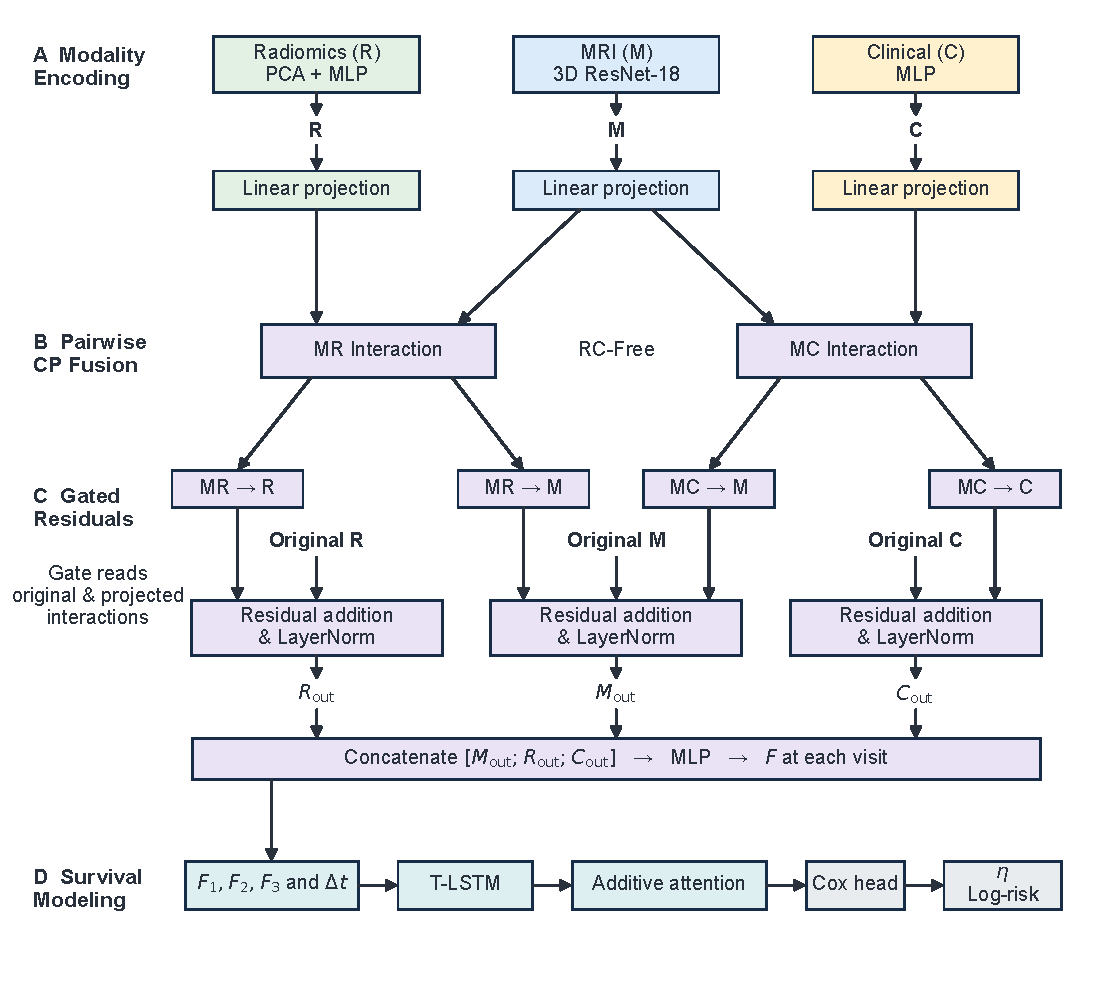
\includegraphics[width=\textwidth]{image_en/final-pipeline.pdf}
\caption{Overall processing pipeline of the proposed RC-Free model}
\label{fig:overall}
\end{figure}
\FloatBarrier

A comprehensive end-to-end schematic spanning raw data curation through survival evaluation is provided in Figure~\ref{fig:master-pipeline}, Appendix~\ref{app:master-pipeline}.

\section{Study Design and Cohort Construction}
\label{sec:study-design}

\subsection{Cohort Selection and the Three-Visit MRI Sequence}
All data analyzed in this study are extracted from the ADNI database \cite{weiner2015impact,jack2008adnimri} across three study phases: ADNI1, ADNIGO, and ADNI2. For each participant (uniquely identified by their Research Identifier, \texttt{RID}), I locate the earliest baseline visit coded as \texttt{bl} with a confirmed diagnosis of MCI (code 2 in the \texttt{DXSUM.DIAGNOSIS} field) \cite{adnidxsum}. Letting $b_i$ denote the baseline visit date, I define the \emph{cohort eligibility milestone} as $L_i = b_i + 18$ calendar months.

To ensure that all individuals enter the post-$L_i$ follow-up period prior to experiencing disease progression, a participant is excluded if they received a dementia diagnosis (code 3 in \texttt{DXSUM.DIAGNOSIS}) \cite{adnidxsum}, recorded an MMSE score $<24$, or had a CDR-global score $\geq 1$ at any time point at or before milestone $L_i$. In addition, each participant is required to have at least one valid cognitive follow-up assessment after $L_i$ to determine the clinical outcome.

Inheriting the three-scan-within-18-months longitudinal design of Aghajanian et al. \cite{aghajanian2025longitudinal}, I select three MRI scans within the observation window $[b_i, L_i]$ after clustering acquisitions separated by at least two months. When multiple scans exist within a single visit cluster, the selection rule prioritizes primary scans over repeat scans and ranks candidates according to ADNI's standardized preprocessing correction tags (prioritizing \texttt{GradWarp + B1 + N3 + Scaled} in ADNI1, and \texttt{GradWarp + N3m} in ADNIGO/ADNI2\footnote{Details on ADNI MRI preprocessing correction levels: \url{https://adni.loni.usc.edu/data-samples/adni-data/neuroimaging/mri/mri-pre-processing/}.}). If a participant has more than three valid scan clusters, the algorithm selects the first scan, the last scan, and the intermediate scan closest to the temporal midpoint, thereby guaranteeing the strict chronological ordering $s_{i1} < s_{i2} < s_{i3} \leq L_i$.

As illustrated in Figure~\ref{fig:cohort}, starting from 899 participants with successfully linked MRI identifiers, this filtering pipeline yields exactly \textbf{359 participants} with 1077 3D MRI volumes (comprising 78 participants from ADNI1, 80 from ADNIGO, and 201 from ADNI2), recording 106 progression events and 253 right-censored cases.

\begin{figure}[H]
\centering
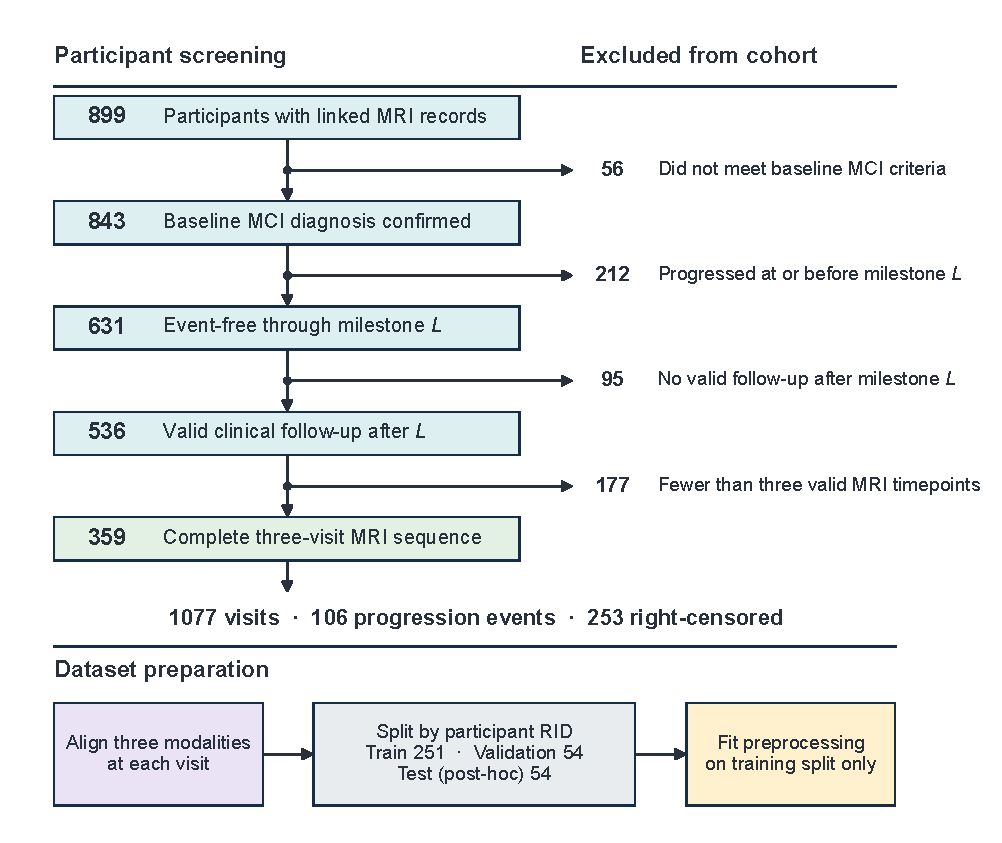
\includegraphics[width=\textwidth]{image_en/cohort-construction.pdf}
\caption{Workflow for longitudinal cohort construction and participant filtering}
\label{fig:cohort}
\end{figure}

\subsection{Outcome Events, Milestones, and Immortal Time Bias}
\label{sec:evaluation-scope}
Following the clinical criteria of Aghajanian et al. \cite{aghajanian2025longitudinal}, a progression event is recorded at the earliest valid clinical visit after milestone $L_i$ that satisfies either MMSE $<24$ or CDR-global $\geq 1$. If a participant never crosses these thresholds through the end of their available follow-up, they are treated as right-censored at their final valid clinical assessment. The survival time $t_i$ (measured in years) is computed from the third MRI scan date ($p_i = s_{i3}$) to the event or censoring date ($o_i$):
\begin{equation}
 t_i=\frac{o_i-p_i}{365.25},\qquad
 \delta_i=\begin{cases}1,&\text{if a progression event is recorded},\\0,&\text{if right-censored}.\end{cases}
 \label{eq:survival-target}
\end{equation}

When analyzing and interpreting Eq.~(\ref{eq:survival-target}), a critical methodological detail to note is the temporal offset between the third MRI scan date $p_i$ and the 18-month eligibility milestone $L_i$. Specifically, among the 359 participants in the cohort, 356 completed their third MRI scan prior to milestone $L_i$, with the gap $L_i - p_i$ having a median of 186 days (interquartile range: 169--197 days). Suppose a participant undergoes their third MRI scan at month 12 ($p_i$) while cohort eligibility is enforced up to month 18 ($L_i$): because the cohort filtering rules exclude all individuals who experienced cognitive decline at or before month 18, any participant retained in the dataset is guaranteed to be event-free between month 12 and month 18. In epidemiology and biostatistics, this guaranteed event-free interval from $p_i$ to $L_i$ is defined as ``immortal time''---a period during which study participants cannot experience the outcome event by design of the inclusion criteria. Including this interval in $t_i$ would induce \emph{immortal time bias} \cite{suissa2008immortal} if the model were interpreted as a prospective forecasting tool deployed immediately at scan date $p_i$. Consequently, all empirical results in this thesis are strictly interpreted for the retrospective risk-ranking task among participants known to have remained stable through milestone $L_i$.

Furthermore, the output $\eta_i$ of the Cox proportional hazards model represents a relative ranking score that orders progression risk across patients. Converting this relative score into an absolute probability of progression (expressed as a percentage at a specific time horizon) for an individual patient requires additionally estimating the baseline cumulative hazard function $H_0(t)$ \cite{cox1972regression}, a point discussed further in Chapter~\ref{chap:discussion}.

\subsection{Dataset Partitioning and Information Leakage Control}
\label{sec:data-split}
A common pitfall in longitudinal medical imaging is splitting individual scans rather than patients across training and evaluation sets; if two visits from the same participant appear in different splits, a model can memorize subject-specific brain anatomy rather than learning generalizable progression patterns. To completely prevent such subject-level leakage, the 359 eligible participants are partitioned strictly by participant identifier (\texttt{RID}) into three mutually exclusive cohorts:
\begin{itemize}[itemsep=0.2em,topsep=0.25em]
\item \emph{Training set} ($N=251$, 74 progression events, 29.5\%): used to optimize all network weights and fit every data-dependent preprocessing statistic.
\item \emph{Validation set} ($N=54$, 16 progression events, 29.6\%): used exclusively for early stopping, hyperparameter tuning, and selecting the final fusion topology.
\item \emph{Post-hoc test set} ($N=54$, 16 progression events, 29.6\%): held out in a locked state until all architectural choices and model checkpoints are finalized, providing an unbiased check of generalization.
\end{itemize}
Stratifying by outcome status preserves a nearly identical event rate (29.5--29.6\%) across all three splits, ensuring that validation and test evaluations reflect comparable censoring proportions.

Equally important is preventing \emph{preprocessing leakage}, which occurs when summary statistics from validation or test subjects influence how training features are scaled or imputed. In this pipeline, every tabular transformation---including the median values used to impute missing clinical scores, the per-feature means and standard deviations used for $z$-score standardization of radiomics and clinical variables, and the Principal Component Analysis (PCA) projection matrix applied to radiomics features---is fitted solely on the 251 training participants. Once fitted, these exact transformation parameters are frozen and applied unchanged to the validation and test sets. Furthermore, the input tensors fed to the model contain only baseline-window imaging, radiomics, and clinical predictors, with no diagnostic labels, event indicators ($\delta_i$), or follow-up durations ($t_i$).

To align multimodal records collected on slightly different clinic dates, each MRI scan is paired with the nearest valid MMSE and CDR assessment within a $\pm 90$-day matching window. Because the third MRI scan date $p_i$ can fall near the end of the 18-month observation window, this symmetric window means that 57 of the 359 participants have an MMSE or CDR score linked to their third MRI that was actually recorded after date $p_i$ (though still strictly prior to the outcome event or censoring date $o_i$). This retrospective matching detail is explicitly noted as a study limitation in Section~\ref{sec:study-limitations}.

Finally, Table~\ref{tab:baseline-characteristics} summarizes the baseline characteristics of all three splits at the first MRI scan, separated by stable ($\delta=0$) and progressing ($\delta=1$) participants. Across the training, validation, and test cohorts, participants have similar ages (mean $\approx 70$--$75$ years), education levels ($\approx 15$--$17$ years), baseline cognitive scores, and inter-visit scan intervals ($s_2-s_1 \approx 120$--$138$ days; $s_3-s_1 \approx 305$--$316$ days). Non-parametric Kruskal--Wallis and $\chi^2$ tests across the three splits all yield $p > 0.05$, confirming that the random participant-level partition produced well-balanced cohorts without systematic demographic or clinical bias.

\begin{landscape}
\begin{table}[p]
\centering\small
\caption[Participant characteristics at the first MRI]{Participant characteristics at the first MRI, stratified by dataset split and outcome status.}
\label{tab:baseline-characteristics}
\setlength{\tabcolsep}{2pt}
\begin{tabular}{@{}lrrrrrrr@{}}
\toprule
& \multicolumn{2}{c}{Training ($N=251$)} & \multicolumn{2}{c}{Validation ($N=54$)} & \multicolumn{2}{c}{Test ($N=54$)} & $p$ \\
\cmidrule(lr){2-3}\cmidrule(lr){4-5}\cmidrule(lr){6-7}
Characteristic & $\delta=0$ & $\delta=1$ & $\delta=0$ & $\delta=1$ & $\delta=0$ & $\delta=1$ & \\
\midrule
Participants & 177 & 74 & 38 & 16 & 38 & 16 & -- \\
Age at first MRI (years) & $71.64 \pm 7.5390$ & $73.41 \pm 7.1692$ & $71.29 \pm 8.6426$ & $74.86 \pm 5.6415$ & $70.03 \pm 7.5755$ & $72.74 \pm 6.7222$ & 0.4895 \\
Male, n (\%) & 96 (54.24) & 49 (66.22) & 23 (60.53) & 10 (62.50) & 28 (73.68) & 9 (56.25) & 0.3367 \\
Education (years) & $16.37 \pm 2.7171$ & $16.61 \pm 2.5846$ & $15.32 \pm 2.5691$ & $17.00 \pm 2.5298$ & $17.00 \pm 2.6304$ & $16.19 \pm 2.9489$ & 0.1465 \\
Baseline MMSE & $28.57 \pm 1.3799$ (53) & $27.22 \pm 1.7746$ (36) & $28.54 \pm 1.1266$ (13) & $27.75 \pm 1.4880$ (8) & $28.25 \pm 1.5275$ (16) & $26.83 \pm 2.0412$ (6) & 0.8688 \\
Baseline CDR-global & $0.44 \pm 0.1613$ (52) & $0.49 \pm 0.0833$ (36) & $0.38 \pm 0.2193$ (13) & $0.44 \pm 0.1768$ (8) & $0.47 \pm 0.1250$ (16) & $0.50 \pm 0.0000$ (6) & 0.2060 \\
Baseline CDR-SB & $0.92 \pm 0.5721$ (52) & $1.68 \pm 0.9573$ (36) & $1.04 \pm 0.8026$ (13) & $1.56 \pm 1.1476$ (8) & $1.28 \pm 0.9123$ (16) & $1.67 \pm 0.9309$ (6) & 0.7260 \\
$s_2-s_1$ (days) & $120.47 \pm 40.5683$ & $134.04 \pm 45.0152$ & $131.76 \pm 41.8372$ & $129.50 \pm 46.4672$ & $124.34 \pm 42.4470$ & $137.50 \pm 44.4627$ & 0.4313 \\
$s_3-s_1$ (days) & $305.12 \pm 44.1559$ & $313.04 \pm 42.8334$ & $307.32 \pm 34.0271$ & $312.19 \pm 75.3819$ & $312.08 \pm 55.0550$ & $315.50 \pm 38.4430$ & 0.8898 \\
$t_i$ (years), mean $\pm$ SD & $5.11 \pm 3.9055$ & $3.41 \pm 2.7858$ & $5.59 \pm 4.7319$ & $3.85 \pm 3.2066$ & $5.51 \pm 4.3420$ & $3.11 \pm 2.5391$ & 0.8713 \\
$t_i$ (years), median [Q1; Q3] & 3.64 [2.02; 7.54] & 2.09 [1.66; 4.42] & 3.92 [2.05; 6.73] & 3.69 [1.44; 4.88] & 4.06 [2.02; 8.20] & 2.42 [1.54; 3.64] & -- \\
\bottomrule
\end{tabular}
\par\vspace{6pt}
\begin{minipage}{0.96\linewidth}\small
$\delta=0$ denotes right-censoring and $\delta=1$ denotes an observed progression event. Unless otherwise noted, values are reported as sample mean $\pm$ SD. For MMSE and CDR, numbers in parentheses indicate the count of valid observations prior to median imputation. Male percentages are computed over participants with available sex records. Age is estimated from birth month and year by assuming the 15th day of the birth month. Demographic variables are taken from the nearest valid record up to the first MRI scan date. MMSE and CDR scores are matched within a $\pm90$-day window. The $p$-values assess differences across the three dataset splits (pooling both outcome statuses) using the Kruskal--Wallis test for continuous variables and the $\chi^2$ test for sex. $s_3-s_1$ denotes the elapsed time from the first to the third MRI scan, and $t_i$ denotes the survival time from the third MRI scan to event or censoring.
\end{minipage}
\end{table}
\end{landscape}


\section{Preprocessing and Modality Encoding}
\label{sec:preprocessing}
Figure~\ref{fig:input-three-sources} illustrates the three information sources linked at each clinical visit prior to entering their respective modality-specific encoders.

\begin{figure}[H]
\centering
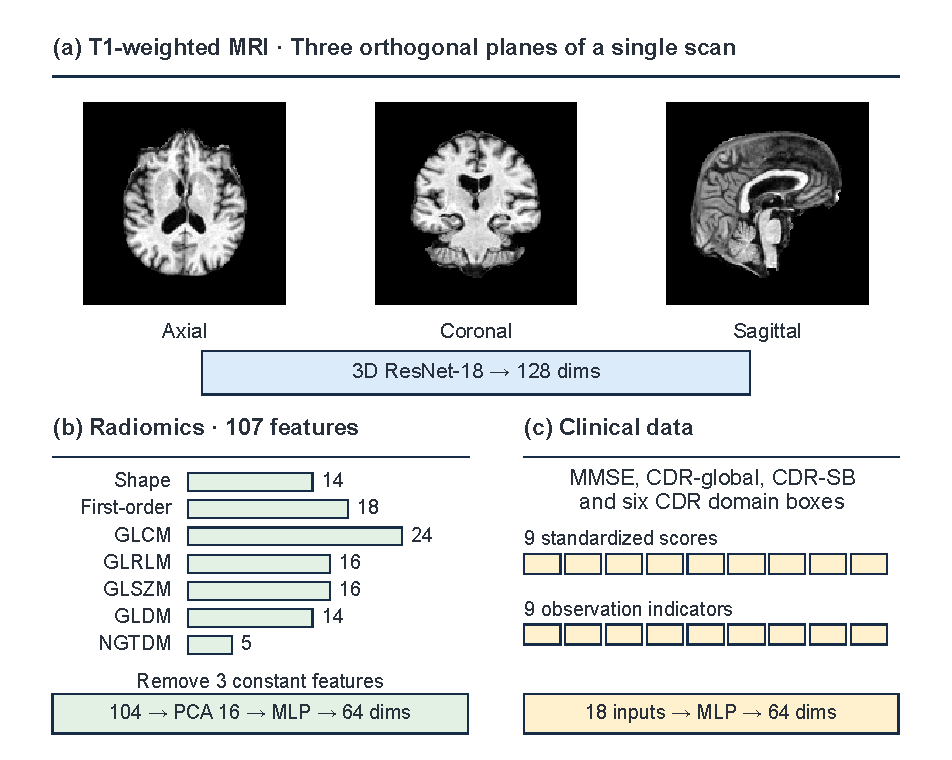
\includegraphics[width=\textwidth]{image_en/input-three-sources.pdf}
\caption[Three input modalities and feature representations]{The three input modalities and their feature representations.}
\label{fig:input-three-sources}
\caption*{\textit{Note.} The three orthogonal MRI planes are extracted by the author from a single preprocessed ADNI T1-weighted volume~\cite{jack2008adnimri}.}
\end{figure}

\subsection{3D MRI Branch and Shared Volumetric Encoder}
In longitudinal 3D brain MRI analysis, even a slight head tilt between consecutive scanning sessions causes the same anatomical structure (such as the hippocampus) to occupy different spatial coordinates, easily leading a neural network to confuse pose shifts with true pathological brain atrophy. Moreover, raw MRI voxel intensities are measured on an arbitrary relative scale that varies across scanners \cite{nyul1999standardizing}. Therefore, I establish a sequential preprocessing pipeline (Figure~\ref{fig:mri-preprocessing}) to standardize spatial orientation, voxel grid geometry, and intensity distribution without distorting the natural anatomical morphology of the brain:

\begin{figure}[H]
\centering
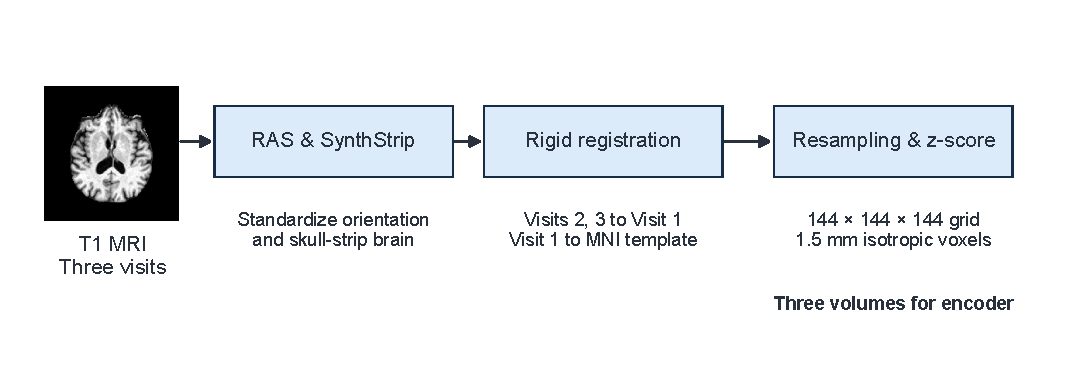
\includegraphics[width=\textwidth]{image_en/mri-preprocessing.pdf}
\caption{Preprocessing pipeline for longitudinal T1-weighted MRI sequences.}
\label{fig:mri-preprocessing}
\caption*{\textit{Note.} The diagram reuses an ADNI slice from Figure~\ref{fig:input-three-sources} to illustrate each step.}
\end{figure}

\begin{enumerate}
\item \emph{Axis reorientation and skull stripping}: All MRI volumes are reoriented to the standard anatomical RAS (\emph{Right--Anterior--Superior}) convention, after which the deep learning tool SynthStrip \cite{hoopes2022synthstrip} removes the skull and scalp tissues and generates a binary whole-brain mask (assigning 1 inside the brain parenchyma and 0 outside, without segmenting gray matter, white matter, or cerebrospinal fluid separately).
\item \emph{Intra-subject and MNI rigid registration}: For each participant, the second and third MRI scans are spatially aligned to that participant's first scan using a 6-degree-of-freedom \emph{rigid registration} (3 translations and 3 rotations, $\mathbf{x}'=\mathbf{R}\mathbf{x}+\mathbf{t}$). Subsequently, the first scan is rigidly aligned to the international standard template MNI152NLin2009cAsym \cite{mcgill2009icbm,fonov2009templates,fonov2011atlases} to establish a common anatomical coordinate frame across all subjects (Figure~\ref{fig:mri-registration}). This pipeline deliberately avoids affine scaling or nonlinear deformable warping so that true inter-subject brain size differences and longitudinal atrophy patterns are preserved intact.
\item \emph{Common grid resampling}: Both the intensity volume and the binary brain mask are resampled onto a uniform $144\times144\times144$ voxel grid with $1.5\text{ mm}$ isotropic resolution, using trilinear interpolation for intensity volumes and nearest-neighbor interpolation for masks to preserve exact binary $0/1$ labels.
\item \emph{Intra-mask intensity standardization}: For each scan independently, voxels inside the whole-brain mask undergo z-score normalization $z(v)=(I(v)-\mu)/\sigma$ (where $\mu$ and $\sigma$ are computed strictly over within-mask voxels of that individual scan) to center the intensity distribution at zero mean and unit variance, while voxels outside the mask are set to zero. No additional N4 bias-field correction is applied so as to preserve the native ADNI correction characteristics.
\end{enumerate}

\begin{figure}[H]
\centering
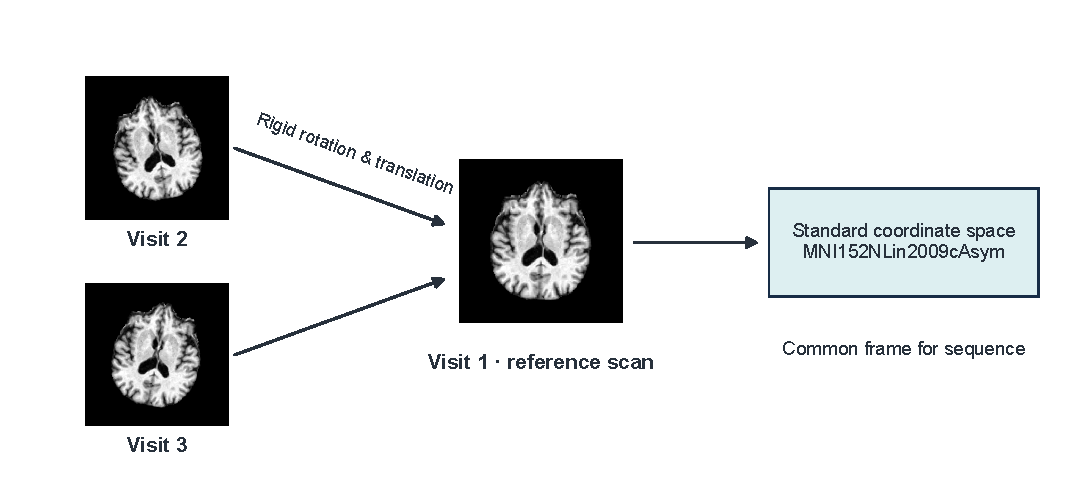
\includegraphics[width=\textwidth]{image_en/mri-registration.pdf}
\caption[Spatial registration across visits and MNI template]{Rigid spatial alignment across visits and to the MNI template.}
\label{fig:mri-registration}
\caption*{\textit{Note.} Poses are illustrated by rotating the same ADNI slice shown in Figure~\ref{fig:input-three-sources}.}
\end{figure}

Following preprocessing, all three MRI volumes of each participant pass through a shared \textbf{3D ResNet-18} encoder implemented in MONAI version 1.5.2\footnote{MONAI source code: \url{https://github.com/Project-MONAI/MONAI/blob/1.5.2/monai/networks/nets/resnet.py}.} \cite{he2016deep,cardoso2022monai}, initialized with complete convolutional weights and BatchNorm statistics pretrained on 3D medical imaging datasets from MedicalNet \cite{chen2019med3d} (with the original classification head removed) and fine-tuned end-to-end from the first training epoch. The backbone consists of four sequential 3D residual stages (with 64, 128, 256, and 512 channels, respectively) using BatchNorm \cite{ioffe2015batchnorm} and ReLU activations \cite{nair2010rectified}. After global average pooling produces a 512-dimensional vector, a linear projection layer ($512\to128$) followed by GELU \cite{hendrycks2016gelu}, Dropout 0.20 \cite{srivastava2014dropout}, and LayerNorm \cite{ba2016layernorm} produces the anatomical representation $M_t\in\mathbb R^{128}$ for each visit. Detailed intermediate feature map dimensions across all layers are listed in Table~\ref{tab:mri-encoder-shapes}, Appendix~\ref{app:mri-shapes}.

\subsection{Radiomics Feature Branch}
\label{sec:radiomics-pipeline}
In parallel with the abstract deep features learned by the 3D CNN, the radiomics branch extracts explicitly defined mathematical descriptors of whole-brain geometry and tissue texture directly from the MRI volume and binary brain mask using the PyRadiomics library \cite{vangriethuysen2017computational}. The extraction pipeline comprises four standardized steps:
\begin{enumerate}
\item \emph{Extraction of 107 features on the $[0,1]$ intensity scale}: Unlike the CNN branch which consumes z-score normalized volumes, the radiomics branch linearly rescales within-mask voxel intensities of each scan to the interval $[0,1]$ and discretizes gray levels using \texttt{binCount=64} \cite{pyradiomicsbins} prior to computing 107 features across 7 families: 3D shape (14 features), first-order intensity statistics (18 features), and five spatial texture matrix families---GLCM, GLRLM, GLSZM, GLDM, and NGTDM (75 features in total), summarized in Table~\ref{tab:radiomics-groups}.
\item \emph{Constant-feature removal}: Because within-mask intensities are rescaled to $[0,1]$, three first-order statistics (\texttt{Minimum}=0, \texttt{Maximum}=1, and \texttt{Range}=1) become constant across all scans and are removed, leaving 104 informative features.
\item \emph{Dimensionality reduction via PCA}: To mitigate severe multicollinearity among the 104 radiomics descriptors, I standardize each variable via z-score normalization and fit a PCA model \cite{jolliffe2016pca} exclusively on the training set with a threshold retaining at least 99\% of the total explained variance, yielding exactly 16 principal components per visit.
\item \emph{MLP encoding}: The 16-dimensional PCA vector passes through a two-layer MLP ($16\to128\to64$) equipped with GELU activation, Dropout 0.20, and LayerNorm to form the radiomics representation $R_t\in\mathbb R^{64}$.
\end{enumerate}

\begin{table}[H]
\centering\small
\caption{Seven radiomics feature families extracted from the 3D MRI volume.}
\label{tab:radiomics-groups}
\begin{tabularx}{\linewidth}{@{}L{2.7cm}r Y Y@{}}
\toprule
Family & Count & Descriptive information & Representative examples \\
\midrule
Shape & 14 & Geometric properties of the whole-brain mask & MeshVolume, SurfaceArea \\
First-order & 18 & Voxel intensity distribution within the mask & Mean, Variance, Entropy \\
GLCM & 24 & Gray-level co-occurrence relationships across voxel pairs & Contrast, Correlation \\
GLRLM & 16 & Run lengths of consecutive voxels sharing a gray level & ShortRunEmphasis, LongRunEmphasis \\
GLSZM & 16 & Sizes of connected homogeneous gray-level zones & SmallAreaEmphasis, LargeAreaEmphasis \\
GLDM & 14 & Gray-level dependency between a voxel and its neighborhood & DependenceEntropy, DependenceVariance \\
NGTDM & 5 & Intensity difference between a voxel and its neighbors & Coarseness, Contrast, Busyness, Complexity, Strength \\
\midrule
Total & 107 & 104 retained after removing Maximum, Minimum, and Range & PCA retains 16 components \\
\bottomrule
\end{tabularx}
\caption*{\textit{Note.} Definitions and representative features follow PyRadiomics~\cite{pyradiomicsfeatures}. Feature counts reflect the extraction catalog of this thesis.}
\end{table}


\subsection{Clinical Data Branch and Missingness Indicators}
The clinical branch leverages 9 prognostic variables (Table~\ref{tab:clinical-inputs}), comprising three composite scores (MMSE-total \cite{folstein1975mmse}, CDR-global, and CDR-SB) and six domain-specific CDR box scores \cite{morris1993cdr}. Any missing values are imputed using the training-set median of that variable at the corresponding visit index (falling back to the global training-set median if an entire visit column is missing), and subsequently standardized using the training-set mean and standard deviation.

Because an imputed value can numerically coincide with an observed clinical measurement, each clinical variable is paired with a \emph{binary observation indicator} (set to 1 if the measurement was actually observed, and 0 if it was missing prior to imputation), expanding the input vector from 9 to 18 dimensions (Figure~\ref{fig:clinical-18}). This 18-dimensional vector passes through a two-layer MLP ($18\to64\to64$) with GELU activation, Dropout 0.10, and LayerNorm to produce the clinical representation $C_t\in\mathbb R^{64}$.

\begin{table}[H]
\centering\small
\caption[Nine input clinical variables]{The nine pre-standardization clinical variables in the exact input order of the model. MMSE follows Folstein et al.~\cite{folstein1975mmse} and CDR follows Morris~\cite{morris1993cdr}. Each variable is paired with a corresponding binary observation indicator.}
\label{tab:clinical-inputs}
\begin{tabularx}{\linewidth}{@{}r L{3.6cm}Y@{}}
\toprule
Index & Clinical variable & Clinical meaning \\
\midrule
1 & MMSE-total & Global cognitive assessment total score, scale 0--30 \\
2 & CDR-global & Overall severity of cognitive and functional impairment \\
3 & CDR-SB & Sum of boxes across the six CDR domains, scale 0--18 \\
4 & CDR: Memory & Ability to retain and recall information \\
5 & CDR: Orientation & Awareness of time, place, and situational context \\
6 & CDR: Judgment & Judgment and problem-solving capability \\
7 & CDR: Community affairs & Independent participation in activities outside the home \\
8 & CDR: Home and hobbies & Ability to perform household tasks and maintain hobbies \\
9 & CDR: Personal care & Degree of independence in personal self-care \\
\bottomrule
\end{tabularx}
\end{table}


\begin{figure}[H]
\centering
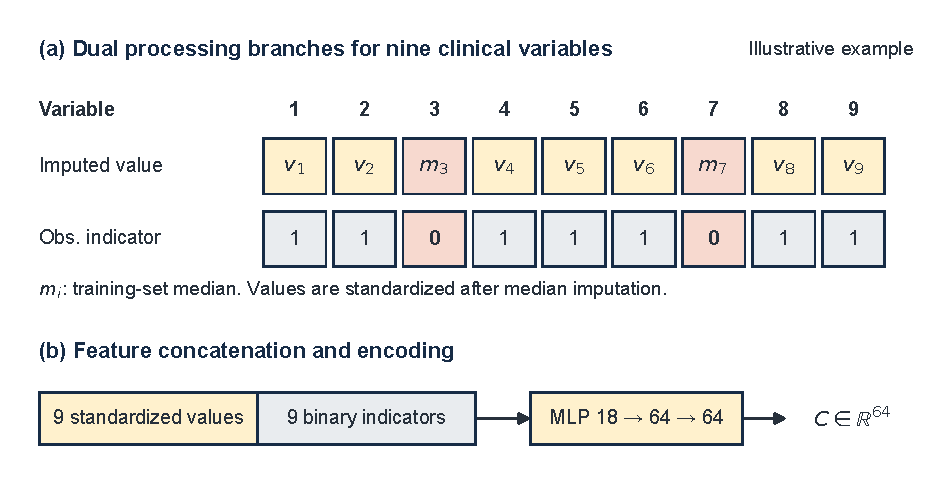
\includegraphics[width=\textwidth]{image_en/clinical-18-inputs.pdf}
\caption{Expanding nine clinical variables into an 18-dimensional input vector}
\label{fig:clinical-18}
\end{figure}

\section{Multimodal Fusion: From Concatenation to RC-Free}
\label{sec:architecture-evolution}
This section presents the systematic progression of the fusion module combining $(M_t, R_t, C_t)$ following the exact empirical verification sequence of this thesis: starting from unimodal MRI reference baselines (Section~\ref{sec:ref-models}), contrasting direct feature concatenation against pairwise outer-product interaction (Section~\ref{sec:pair-fusion}), compressing bilinear layers via CP tensor decomposition (Section~\ref{sec:cp-method}), and culminating in the dynamically gated residual routing mechanism and the streamlined RC-Free topology (Section~\ref{sec:gated-routing}).

\subsection{Reference Baselines on MRI Data}
\label{sec:ref-models}
To isolate the added value of longitudinal temporal dynamics and establish a rigorous benchmark against prior literature, this thesis constructs a sequence of unimodal MRI baselines (comprising a single-timepoint Last-MRI model, a 3-visit longitudinal MRI model with T-LSTM, and a longitudinal MRI model combining T-LSTM with additive attention) alongside an adapted re-implementation of the CNN--PCA--T-LSTM pipeline of Aghajanian et al. \cite{aghajanian2025longitudinal}. In this adapted re-implementation, a TensorFlow CNN processes $128^3$ MRI volumes and outputs 512-dimensional feature vectors; a PCA transform is fitted on the training set to retain 99\% variance (without feature scaling or whitening) before feeding a T-LSTM with a 64-dimensional hidden state. Table~\ref{tab:reference-methods} delineates the exact similarities and differences among the original published study, the adapted re-implementation, and the primary RC-Free model of this thesis. All primary models are implemented in PyTorch, MONAI, and scikit-learn \cite{paszke2019pytorch,cardoso2022monai,pedregosa2011sklearn}; differences in optimizer and batch size in the CNN--PCA--T-LSTM re-implementation are benchmarked on a unified basis via the validation C-index.

\begin{table}[H]
\centering\small
\caption[Comparison across the three methodologies]{Comparison of cohort data, configurations, and roles across methodologies.}
\label{tab:reference-methods}
\begin{tabularx}{\textwidth}{@{}L{3.2cm}Y Y@{}}
\toprule
\textbf{Methodology} & \textbf{Cohort and Preprocessing} & \textbf{Architecture and Role} \\
\midrule
Original Aghajanian \cite{aghajanian2025longitudinal} & 228 MCI subjects; SPM12, gray-matter volumes and gray-matter radiomics & CNN--PCA--T-LSTM; two-stage training; literature reference baseline \\
Adapted re-implementation & 359 subjects; MRI volumes resized to fixed $128^3$ grid & Per-seed CNN/PCA; 64-d T-LSTM; implementation benchmark \\
RC-Free Pairwise & 359 subjects; $144^3$ MRI, whole-brain radiomics, 18-d clinical input & MedicalNet; CP MR/MC; gated residuals; 128-d T-LSTM; primary proposed model \\
\bottomrule
\end{tabularx}
\end{table}

\subsection{Concatenation Baseline and Full Outer-Product Fusion}
\label{sec:pair-fusion}
When combining all three modality representations $(M_t\in\mathbb R^{128}, R_t\in\mathbb R^{64}, C_t\in\mathbb R^{64})$ simultaneously, the most direct baseline is \textbf{feature concatenation (Concatenation)}: keeping all three modality encoders unchanged, concatenating the three vectors directly into a 256-dimensional vector, and passing it through $\operatorname{MLP}_{\rm out}$ (a linear projection $256\to128$ followed by GELU, Dropout 0.20, and LayerNorm) to produce the visit representation $F_t\in\mathbb R^{128}$ for the temporal block (Figure~\ref{fig:concat-baseline}):
\begin{equation}
 F_t=\operatorname{MLP}_{\rm out}(M_t\concat R_t\concat C_t),\qquad
 M_t\concat R_t\concat C_t\in\mathbb R^{256},\quad F_t\in\mathbb R^{128}.
 \label{eq:concat}
\end{equation}

\begin{figure}[H]
\centering
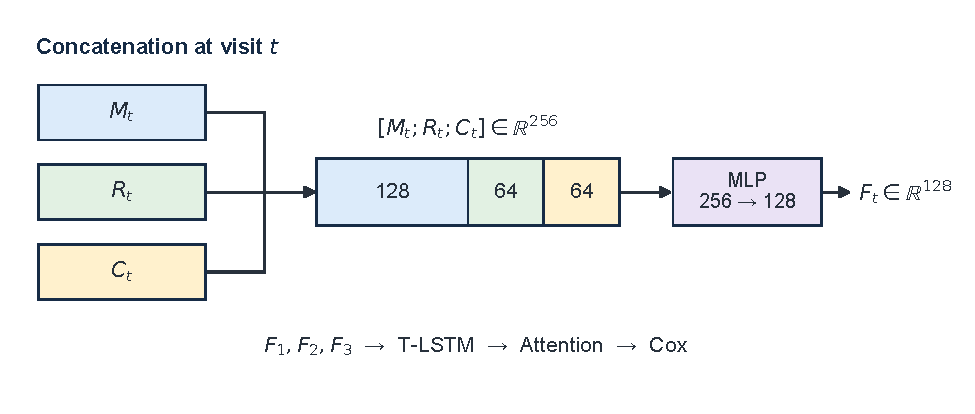
\includegraphics[width=\textwidth]{image_en/concat-baseline.pdf}
\caption[Three-modality concatenation baseline]{Computational flow of the three-modality concatenation baseline.}
\label{fig:concat-baseline}
\end{figure}

Under pure concatenation, discovering cross-modal relationships is left entirely to downstream projection layers. To overcome this limitation and explicitly capture bilinear interactions between modality pairs right before the concatenation step in Eq.~(\ref{eq:concat}), I construct the \textbf{Full Outer-Product} variant, which introduces three pairwise bilinear interaction modules: MR, MC, and RC. First, three bias-free linear projections reduce the dimensionality of each original modality representation to keep the outer-product space tractable:
\begin{equation}
 \widetilde M\in\mathbb R^{32},\qquad
 \widetilde R\in\mathbb R^{32},\qquad
 \widetilde C\in\mathbb R^{16}.
 \label{eq:input-projection}
\end{equation}

For each pair $k\in\{\mathrm{MR},\mathrm{MC},\mathrm{RC}\}$, let $x\in\mathbb R^{d_x}$ and $y\in\mathbb R^{d_y}$ denote the two dimension-reduced input vectors. The model computes the outer-product matrix $xy^\top \in \mathbb R^{d_x\times d_y}$, flattens it into a vector (1024 dimensions for MR; 512 dimensions for MC and RC), and passes it through a two-layer MLP equipped with GELU, Dropout 0.10, and LayerNorm (with layer dimensions MR: $1024\to128\to64$; MC: $512\to128\to64$; and RC: $512\to64\to32$), as illustrated in Figure~\ref{fig:mr-outer-product}. When all three pairwise modules are active, six routing branches project the resulting interaction representations back to the dimensionality of each constituent target modality to residually enrich the original representations prior to entering $\operatorname{MLP}_{\rm out}$ (Figure~\ref{fig:pair-update-routes}).

\begin{figure}[H]
\centering
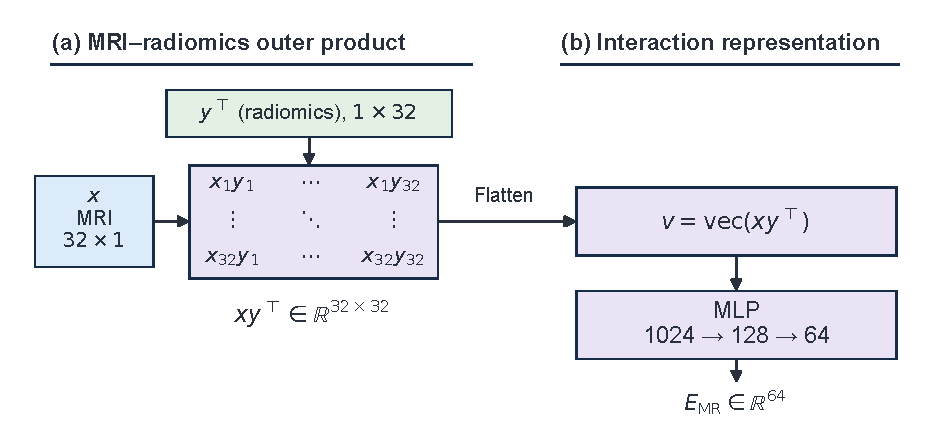
\includegraphics[width=\textwidth]{image_en/mr-outer-product.pdf}
\caption{Full outer-product and interaction MLP block (MR pair)}
\label{fig:mr-outer-product}
\end{figure}

\begin{figure}[H]
\centering
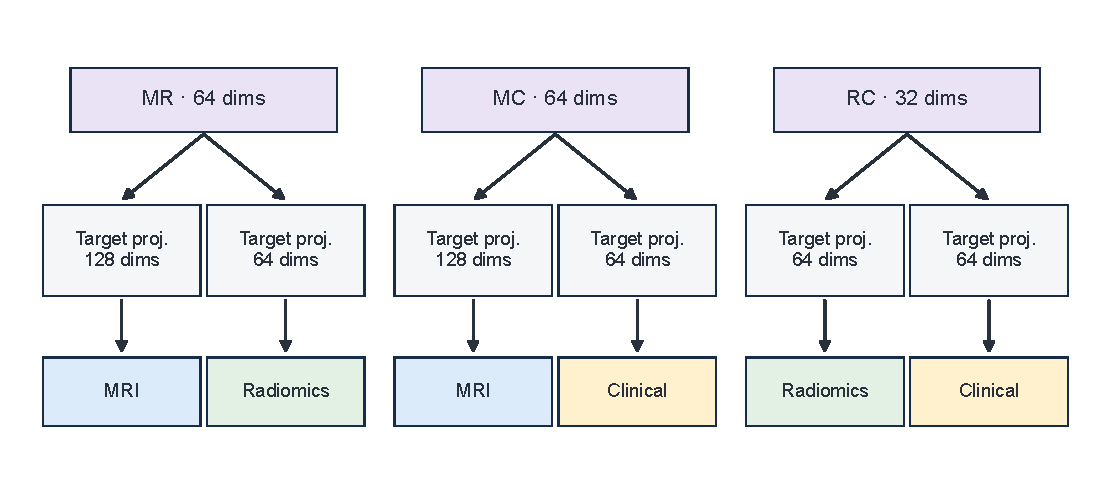
\includegraphics[width=\linewidth]{image_en/pair-update-routes.pdf}
\caption{Six update routing branches from three pairwise interactions}
\label{fig:pair-update-routes}
\end{figure}

\subsection{CP Tensor Parameter Compression}
\label{sec:cp-method}
As analyzed in Section~\ref{sec:background-fusion}, the initial linear projection layer immediately following an outer product corresponds to a third-order weight tensor $\mathcal W\in\mathbb R^{d_h\times d_x\times d_y}$ requiring $d_h d_x d_y + d_h$ parameters, which is highly prone to overfitting on a training cohort of 251 patients. To eliminate this bottleneck, I apply rank-$Q$ CP tensor decomposition according to Eqs.~(\ref{eq:cp-concept-math})--(\ref{eq:cp-hadamard}) \cite{carroll1970candecomp,kolda2009tensor,liu2018lowrank}: the initial bilinear layer of each interaction pair $k$ is replaced by three low-rank factor matrices $A\in\mathbb R^{d_x\times Q}$, $B\in\mathbb R^{d_y\times Q}$ (without bias), and $O\in\mathbb R^{d_h\times Q}$ (with bias vector $b$):
\begin{align}
 u&=A^\top x,\qquad v=B^\top y,\qquad q=u\odot v,\label{eq:cp-lowrank}\\
 h&=Oq+b,\qquad E_k=\operatorname{PostMLP}_k(h).
 \label{eq:cpblock}
\end{align}
Here, $\operatorname{PostMLP}_k$ retains the exact downstream architecture consisting of GELU activation, Dropout 0.10, a linear layer $d_h\to d_o$, and LayerNorm, outputting the pairwise interaction vector $E_k\in\mathbb R^{d_o}$ for pair $k\in\{\mathrm{MR},\mathrm{MC},\mathrm{RC}\}$ (specifically $E_{\mathrm{MR}}\in\mathbb R^{64}$, $E_{\mathrm{MC}}\in\mathbb R^{64}$, and $E_{\mathrm{RC}}\in\mathbb R^{32}$). This design guarantees a strictly fair experimental comparison: the CP variant modifies only the initial bilinear projection layer (Figure~\ref{fig:cp-block}) while keeping every subsequent layer identical to Full Outer-Product. The parameter count of the initial bilinear layer is thereby compressed from $d_h d_x d_y + d_h$ down to $Q(d_x+d_y+d_h)+d_h$. Table~\ref{tab:cpconfig} summarizes the dimensional configuration and CP rank for each pair (setting $Q=8$ for MR and MC, and $Q=4$ for RC due to its smaller output dimension).

\begin{figure}[H]
\centering
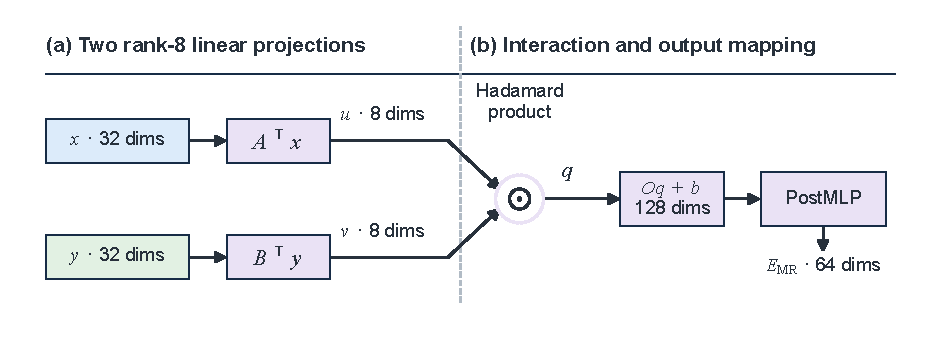
\includegraphics[width=\textwidth]{image_en/outer-vs-cp.pdf}
\caption{Rank-$Q=8$ CP interaction block for the MR pair}
\label{fig:cp-block}
\end{figure}

\begin{table}[H]
\centering\small
\caption{Dimensional configuration and CP rank across pairwise interaction modules}
\label{tab:cpconfig}
\begin{tabular}{lccccc}
\toprule
Pair & $(d_x,d_y)$ & Rank $Q$ & Hidden dim $d_h$ & Output dim $d_o$ & RC-Free \\
\midrule
MR & $(32,32)$ & 8 & 128 & 64 & Retained \\
MC & $(32,16)$ & 8 & 128 & 64 & Retained \\
RC & $(32,16)$ & 4 & 64 & 32 & Pruned \\
\bottomrule
\end{tabular}
\end{table}

\subsection{Gated Residual Routing and the Streamlined RC-Free Topology}
\label{sec:gated-routing}
\label{sec:rcfree-method}
Once the bilinear interaction representation $E_k\in\mathbb R^{d_o}$ has been extracted from each pair $k$ via Eq.~(\ref{eq:cpblock}), the next crucial step is routing this interaction information back to enrich the original representations of the two constituent modalities. Let $U_d$ denote the original representation of target modality $d\in\{M,R,C\}$ (i.e., $U_M=M\in\mathbb R^{128}$, $U_R=R\in\mathbb R^{64}$, and $U_C=C\in\mathbb R^{64}$). Because cross-modal interactions are not equally reliable across all patients or visits (for example, when an MRI scan suffers from motion artifacts or when clinical scores are imputed from missing entries), the proposed model does not add $E_k$ directly; instead, it routes the signal through a dynamically gated residual branch $k\to d$ comprising three sequential components (Figure~\ref{fig:route}):
\begin{enumerate}
\item \emph{Projecting $E_k$ into a target-aligned interaction vector $\widehat E_{k\to d}$}: The shared interaction vector $E_k$ cannot be added directly to the original representation $U_d$, first because of dimensional mismatch (for instance, $E_{\mathrm{MR}}$ has 64 dimensions whereas the target MRI representation $U_M$ has 128 dimensions), and second because the two constituent modalities in a pair need to extract distinct complementary cues from $E_k$. Therefore, on each routing branch $k\to d$, I apply a dedicated linear projection $W_{k\to d}$ (with bias $b_{k\to d}$ and no nonlinear activation) followed by LayerNorm to transform $E_k$ into a target-aligned interaction vector $\widehat E_{k\to d}$ matching the exact dimensionality of $U_d$:
\begin{equation}
 \widehat E_{k\to d}=\LN_{k\to d}(W_{k\to d}E_k+b_{k\to d}).
 \label{eq:target-projection}
\end{equation}
\item \emph{Sample-adaptive dynamic gate $g_{k\to d}\in(0,1)$}: The gating unit receives both the layer-normalized original representation and the target-aligned interaction vector simultaneously to determine a visit-specific opening weight through a 32-dimensional hidden MLP (initialized via Xavier uniform initialization \cite{glorot2010understanding} with zero initial biases) terminated by a sigmoid activation:
\begin{equation}
 g_{k\to d}=\sigma\!\left(
 w_{k\to d}^{\top}\operatorname{GELU}\!\left[
 V_{k\to d}\bigl(\LN_d^{\rm gate}(U_d)\concat\widehat E_{k\to d}\bigr)
 +a_{k\to d}\right]+c_{k\to d}\right).
 \label{eq:dynamic-gate}
\end{equation}
Using an independent sigmoid gate for each branch (rather than a softmax gate constrained to sum to 1) allows multiple branches to open concurrently when complementary signals are informative, or close toward 0 simultaneously when noise is detected.
\item \emph{Global scaling coefficient $\lambda_{k\to d}$}: A learnable scalar parameter shared across the dataset (initialized at $0.1$ without sign constraints) that modulates the overall amplitude and polarity of each routing branch.
\end{enumerate}

\begin{figure}[H]
\centering
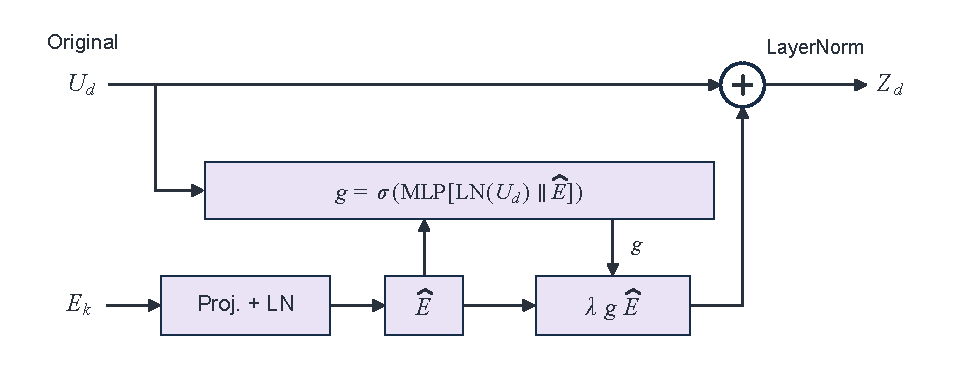
\includegraphics[width=\textwidth]{image_en/gated-residual-route.pdf}
\caption{Architecture of a single dynamically gated residual routing branch}
\label{fig:route}
\end{figure}

The updated representation of target modality $d$, after accumulating gated residuals from its set of active interaction pairs $\mathcal P(d)$, is normalized via a dedicated output LayerNorm:
\begin{equation}
 Z_d=\LN_d^{\rm out}\!\left(
 U_d+\sum_{k\in\mathcal P(d)}\lambda_{k\to d}\,g_{k\to d}\,\widehat E_{k\to d}
 \right).
 \label{eq:ours-residual}
\end{equation}
The three LayerNorm instances in Eqs.~(\ref{eq:target-projection})--(\ref{eq:ours-residual}) maintain completely independent parameter sets \cite{ba2016layernorm}. Whenever the dynamic gate $g_{k\to d}$ approaches 0, the interaction branch is effectively silenced and the output faithfully preserves the normalized original representation $\LN_d^{\rm out}(U_d)$.

The standard Full CP model maintains all three interaction pairs (MR, MC, and RC) along with all six residual routing branches. However, because radiomics features are mathematically extracted directly from the MRI volume itself, maintaining an additional direct interaction between radiomics and clinical scores (the RC pair) introduces potential representational redundancy once MRI is already directly coupled with both modalities. Motivated by this insight, I propose the streamlined \textbf{RC-Free} architecture: completely pruning the RC interaction module and positioning MRI as the central hub connecting the MR and MC pairs (both with decomposition rank $Q=8$), thereby reducing the number of gated residual routing branches from six to four while preserving all three input modalities (Figure~\ref{fig:rcfree-update}).

\begin{figure}[H]
\centering
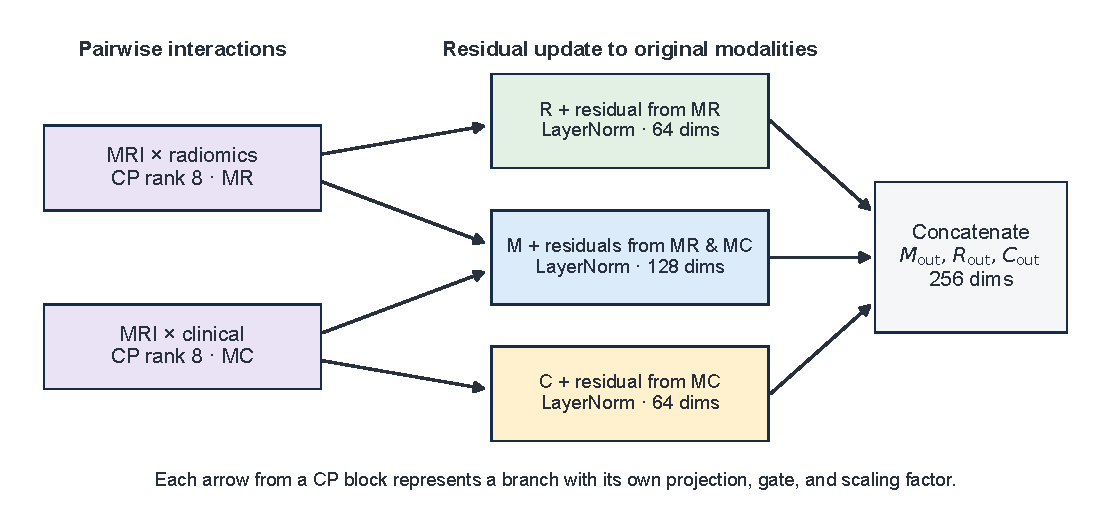
\includegraphics[width=\linewidth]{image_en/rcfree-update.pdf}
\caption{Four feature update routing branches in the proposed RC-Free architecture}
\label{fig:rcfree-update}
\end{figure}

Letting $D_{k\to d}=\lambda_{k\to d}\,g_{k\to d}\,\widehat E_{k\to d}$, the three updated modality representations in RC-Free take the explicit form:
\begin{align}
 M_{\rm out}&=\LN_M^{\rm out}(M+D_{(\mathrm{MR}\to M)}+D_{(\mathrm{MC}\to M)}),\label{eq:rcfree-first}\\
 R_{\rm out}&=\LN_R^{\rm out}(R+D_{(\mathrm{MR}\to R)}),\\
 C_{\rm out}&=\LN_C^{\rm out}(C+D_{(\mathrm{MC}\to C)}).
 \label{eq:rcfree-residual}
\end{align}
The three updated vectors $M_{\rm out}\in\mathbb R^{128}$, $R_{\rm out}\in\mathbb R^{64}$, and $C_{\rm out}\in\mathbb R^{64}$ are then concatenated into a 256-dimensional vector and projected through the same $\operatorname{MLP}_{\rm out}$ layer ($256\to128$, identical to Eq.~(\ref{eq:concat})) to obtain the fused visit representation $F_t\in\mathbb R^{128}$ at visit $t$. By keeping this 128-dimensional output interface fixed, varying the active set of pairwise interactions requires no changes to the downstream temporal modeling or survival prediction layers.

\section{Temporal Modeling and Cox Objective}
\label{sec:temporal-method}
\label{sec:training-method}
The sequence of three fused visit representations $F_t\in\mathbb R^{128}$ ($t=1,2,3$) together with the actual elapsed time intervals between consecutive scans $\Delta t_t=(s_t-s_{t-1})/365.25$ (measured in years, with $\Delta t_1=0$ by convention) is fed into a single-layer unidirectional temporal modeling block (Figure~\ref{fig:temporal}).

Adopting the T-LSTM formulation of Baytas et al. \cite{baytas2017patient} with a 128-dimensional hidden state, at time step $t$, the previous cell memory $c_{t-1}$ is decomposed into a short-term memory component $c_{t-1}^{S}$ (discounted by a monotonically decreasing decay weight $\gamma_t$ as $\Delta t_t$ increases) and a sustained long-term memory component $c_{t-1}^{L}$:
\begin{align}
 c_{t-1}^{S}&=\tanh(W_Sc_{t-1}+b_S),\qquad
 c_{t-1}^{L}=c_{t-1}-c_{t-1}^{S},\label{eq:tlstm-first}\\
 \gamma_t&=\frac{1}{\log(e+\Delta t_t)},\qquad
 c_{t-1}^{*}=c_{t-1}^{L}+\gamma_t c_{t-1}^{S}.
 \label{eq:tlstm-memory}
\end{align}
The time-adjusted memory state $c_{t-1}^{*}$ then enters the standard LSTM forget gate $f_t$, input gate $i_t$, output gate $o_t$, and candidate memory $\widetilde c_t$ equations (computed from $F_t$ and $h_{t-1}$):
\begin{equation}
 c_t=f_t\odot c_{t-1}^{*}+i_t\odot\widetilde c_t,
 \qquad h_t=o_t\odot\tanh(c_t).
 \label{eq:tlstm-state}
\end{equation}
(If a visit were flagged as invalid, the recurrent cell would carry forward its previous state; in our curated cohort, all three visits of every participant are valid.)

\begin{figure}[H]
\centering
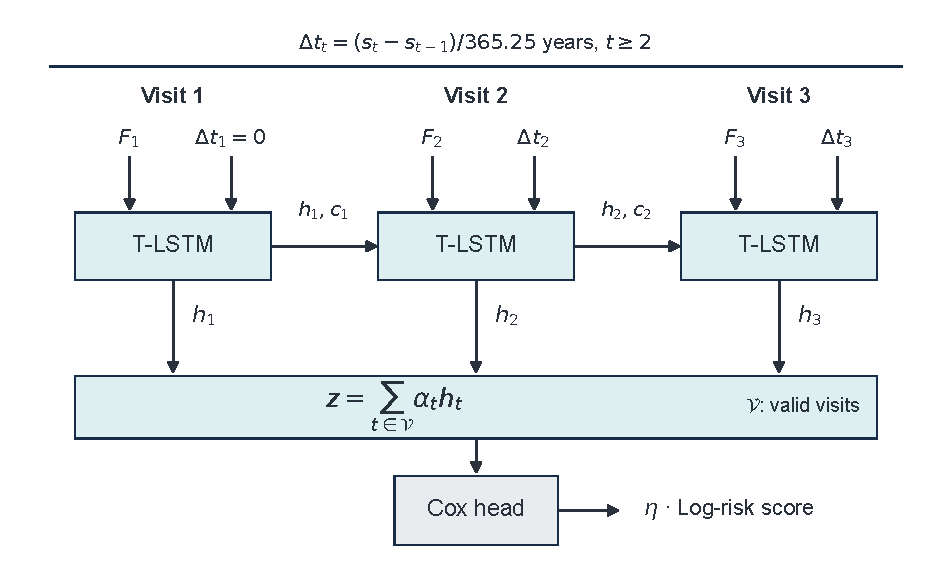
\includegraphics[width=\textwidth]{image_en/temporal-model.pdf}
\caption{Temporal T-LSTM block, additive attention, and Cox head}
\label{fig:temporal}
\end{figure}

Next, an additive attention mechanism (Eq.~(\ref{eq:additive-attention}) following Yang et al. \cite{yang2016hierarchical}) applies a $128\to64\to1$ scoring network to assign normalized importance weights $\alpha_t$ across the set of valid visits $\mathcal V$:
\begin{equation}
 e_t=v_a^\top\tanh(W_a h_t+b_a),\qquad
 \alpha_t=\frac{\exp(e_t)}{\sum_{j\in\mathcal V}\exp(e_j)},\qquad
 z=\sum_{t\in\mathcal V}\alpha_t h_t.
 \label{eq:temporal-attention}
\end{equation}
From the aggregated longitudinal representation $z\in\mathbb R^{128}$, an output MLP head ($128\to64$ with GELU activation and Dropout 0.30, followed by a linear layer $64\to1$) estimates the scalar log-risk score $\eta_i\in\mathbb R$ in the Cox proportional hazards model of Eq.~(\ref{eq:cox-hazard}). The entire network is trained end-to-end by minimizing the negative Cox partial log-likelihood (Eq.~(\ref{eq:cox-loss})) averaged over the $N_e$ observed events in a batch, handling tied event times via Breslow's approximation \cite{breslow1974covariance}:
\begin{equation}
 \mathcal L_{\rm Cox}=-\frac{1}{N_e}\sum_k
 \left[\sum_{i\in\mathcal D_k}\eta_i
 -d_k\log\!\left(\sum_{j\in\mathcal R_k}\exp(\eta_j)\right)\right],
 \label{eq:cox-method}
\end{equation}
where $\mathcal D_k$ denotes the set of individuals experiencing an event at distinct event time $\tau_k$ ($d_k=|\mathcal D_k|$) and $\mathcal R_k=\{j:t_j\geq\tau_k\}$ is the risk set at time $\tau_k$. The complete forward pass of the proposed RC-Free model is summarized in Algorithm~\ref{alg:rcfree-forward}.

\begin{algorithm}[H]
\caption{Forward pass of the RC-Free Pairwise Fusion model}
\label{alg:rcfree-forward}
\small
\textbf{Input:} A longitudinal sequence of three visits $(t=1,2,3)$ for an individual, consisting of preprocessed 3D MRI volumes, PCA-compressed radiomics feature vectors (16 dimensions), clinical vectors comprising nine standardized scores and nine observation indicators (18 dimensions), and elapsed inter-visit intervals $\Delta t_t$ (with $\Delta t_1=0$).\\
\textbf{Output:} Individual log-risk score $\eta\in\mathbb R$.
\begin{enumerate}[leftmargin=1.2em,label=\arabic*.,itemsep=0.2em]
\item For each visit $t=1,2,3$:
\begin{enumerate}[leftmargin=1.2em,label=\alph*.,itemsep=0.15em]
\item Encode the three input sources at visit $t$ into $M_t\in\mathbb R^{128}$, $R_t\in\mathbb R^{64}$, and $C_t\in\mathbb R^{64}$ as detailed in Section~\ref{sec:preprocessing}; apply bias-free linear projections to obtain reduced representations $\widetilde M_t\in\mathbb R^{32}$, $\widetilde R_t\in\mathbb R^{32}$, and $\widetilde C_t\in\mathbb R^{16}$ via Eq.~(\ref{eq:input-projection}).
\item Compute pairwise interaction representations $E_{\mathrm{MR},t}\in\mathbb R^{64}$ from $(\widetilde M_t,\widetilde R_t)$ and $E_{\mathrm{MC},t}\in\mathbb R^{64}$ from $(\widetilde M_t,\widetilde C_t)$ using two rank-$Q=8$ CP interaction blocks followed by their respective MLPs according to Eqs.~(\ref{eq:cp-lowrank})--(\ref{eq:cpblock}).
\item For each active routing branch $k\to d\in\{\mathrm{MR}\to M,\mathrm{MR}\to R,\mathrm{MC}\to M,\mathrm{MC}\to C\}$, compute the target-aligned projection $\widehat E_{k\to d,t}$ via Eq.~(\ref{eq:target-projection}), the dynamic gating coefficient $g_{k\to d,t}$ via Eq.~(\ref{eq:dynamic-gate}), and the gated residual update $D_{k\to d,t}=\lambda_{k\to d}\,g_{k\to d,t}\,\widehat E_{k\to d,t}$.
\item Apply residual updates and layer normalization according to Eqs.~(\ref{eq:rcfree-first})--(\ref{eq:rcfree-residual}) to obtain $M_{\mathrm{out},t}\in\mathbb R^{128}$, $R_{\mathrm{out},t}\in\mathbb R^{64}$, and $C_{\mathrm{out},t}\in\mathbb R^{64}$.
\item Concatenate the updated modality vectors and project them into the fused visit representation: $F_t=\operatorname{MLP}_{\mathrm{out}}(M_{\mathrm{out},t}\concat R_{\mathrm{out},t}\concat C_{\mathrm{out},t})\in\mathbb R^{128}$ via Eq.~(\ref{eq:concat}).
\end{enumerate}
\item Initialize hidden and cell states to zero; pass the temporal sequence $(F_t,\Delta t_t)_{t=1}^3$ through the T-LSTM cell according to Eqs.~(\ref{eq:tlstm-first})--(\ref{eq:tlstm-state}) to obtain hidden states $h_1,h_2,h_3\in\mathbb R^{128}$.
\item Compute additive attention weights $\alpha_t$ and the aggregated longitudinal representation $z=\sum_{t=1}^3\alpha_t h_t\in\mathbb R^{128}$ via Eq.~(\ref{eq:temporal-attention}).
\item Pass $z$ through the Cox survival prediction MLP head ($128\to64\to1$) described in Section~\ref{sec:training-method} to output the scalar log-risk score $\eta$.
\end{enumerate}
\end{algorithm}


\section{Risk Ranking and Survival Stratification Evaluation}
\label{sec:survival-evaluation}
A prognostic survival model must be evaluated simultaneously across three complementary dimensions (Figure~\ref{fig:evaluation-map}): global ranking concordance (C-index), longitudinal risk-group stratification (Kaplan--Meier curves), and time-horizon-specific discrimination (IPCW-AUC). All evaluations are computed on the out-of-sample risk scores $\eta_i$ generated by the three frozen RC-Free checkpoints (corresponding to the three random initializations).

\begin{figure}[H]
\centering
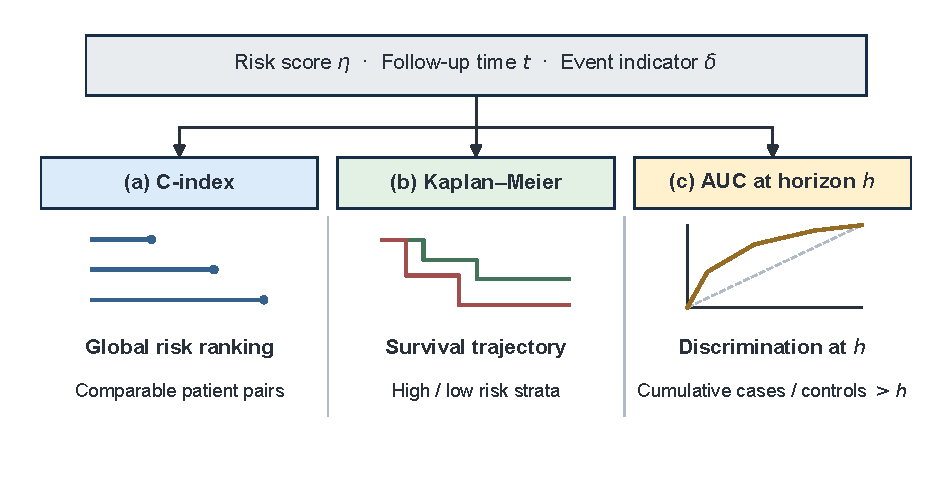
\includegraphics[width=\textwidth]{image_en/evaluation-map.pdf}
\caption{Three evaluation perspectives for survival risk ranking and stratification}
\label{fig:evaluation-map}
\end{figure}

\subsection{Harrell's Concordance Index (C-index)}
Harrell's C-index \cite{harrell1996multivariable} measures the proportion of comparable participant pairs ($t_i<t_j$ with $\delta_i=1$) in which the model correctly assigns a higher risk score to the individual who experiences the progression event earlier ($\eta_i>\eta_j$). A value of 0.5 corresponds to random guessing and 1.0 indicates perfect concordance. The validation set contains 480 comparable pairs and the post-hoc test set contains 528 comparable pairs; results are reported as sample mean $\pm$ standard deviation (SD) across the three random initializations.

\subsection{Kaplan--Meier Stratification via Consensus Risk Groups}
To verify whether the continuous risk score $\eta_i$ can separate patients into clinically distinct progression trajectories, I use the \emph{training-set median risk score} as a fixed cutoff threshold (strictly avoiding any threshold optimization on the validation or test sets): individuals scoring above the threshold are assigned to the high-risk group, and those at or below the threshold are assigned to the low-risk group. To reduce sensitivity to any single random initialization, the final group assignment for each participant is determined by \emph{majority-vote consensus} across the three seeds (assigning a participant to the high-risk group if at least 2 out of 3 seeds classify them as high-risk).

Given the resulting high- and low-risk groups, Kaplan--Meier survival curves \cite{kaplan1958nonparametric} estimate the probability of remaining event-free over time, plotted with 95\% confidence intervals, right-censoring ticks, and numbers at risk at 0, 2, 3, and 5 years. Separation between the two survival curves is tested via the nonparametric log-rank test \cite{mantel1966survival}, while a univariate Cox regression model estimates the hazard ratio (HR) and its 95\% confidence interval across the entire follow-up duration. The proportional hazards (PH) assumption is verified using scaled Schoenfeld residuals following Grambsch and Therneau \cite{grambsch1994proportional} (with rank-transformed time).

\subsection{IPCW Time-Dependent AUC at 2, 3, and 5 Years}
At each clinical evaluation horizon $h \in \{2, 3, 5\text{ years}\}$, I evaluate the model's ability to discriminate between cumulative cases up to horizon $h$ ($\mathcal C_h=\{i:\delta_i=1,t_i\leq h\}$) and dynamic controls who remain event-free beyond $h$ ($\mathcal D_h=\{j:t_j>h\}$) using the cumulative/dynamic AUC estimator \cite{hung2010time}. Because participants right-censored prior to $h$ have unknown event status at horizon $h$, naively omitting them would introduce censoring bias; therefore, each event case is weighted by the inverse probability of censoring $w_i = 1/\widehat G(t_i)$ (IPCW) \cite{polsterl2020scikit,hung2010time}, where the censoring survival distribution $\widehat G(\cdot)$ is estimated via the Kaplan--Meier method on the training set under the assumption of independent censoring \cite{sksurvauc}:
\begin{equation}
 \widehat{\operatorname{AUC}}(h)=
 \frac{\displaystyle\sum_{i\in\mathcal C_h}w_i
 \sum_{j\in\mathcal D_h}\kappa(\eta_i,\eta_j)}
 {\displaystyle |\mathcal D_h|\sum_{i\in\mathcal C_h}w_i},
 \qquad
 \kappa(a,b)=\begin{cases}
 1,&a>b,\\
 \tfrac12,&a=b,\\
 0,&a<b.
 \end{cases}
 \label{eq:ipcw-auc}
\end{equation}
Following the standard implementation in \texttt{scikit-survival}, two risk scores differing by no more than $10^{-8}$ are treated as tied \cite{sksurvauc}. To avoid extrapolating the training censoring distribution when the maximum follow-up time in the validation set (18.26 years) exceeds that of the training set (13.95 years), evaluation times are capped at $h+\varepsilon$ (determined via \texttt{nextafter}).
